\documentclass[10pt,aspectratio=169]{beamer}

%\usepackage{pgfpages}
%\pgfpagesuselayout{4 on 1}[letterpaper,landscape,border shrink=5mm]

\usetheme{Madrid}
\definecolor{Pantone295}{rgb}{0, 0.15686, 0.33333} % Pantone 295 (primary)
\definecolor{UBCgrey}{rgb}{0.3686, 0.5255, 0.6235} % UBC Grey (secondary)
\setbeamercolor{palette primary}{bg=Pantone295,fg=white}
\setbeamercolor{palette secondary}{bg=Pantone295,fg=white}
\setbeamercolor{palette tertiary}{bg=Pantone295,fg=white}
\setbeamercolor{palette quaternary}{bg=Pantone295,fg=white}
\setbeamercolor{structure}{fg=Pantone295} % itemize, enumerate, etc
\setbeamercolor{section in toc}{fg=Pantone295} % TOC sections
% Override palette coloring with secondary
\setbeamercolor{subsection in head/foot}{bg=UBCgrey,fg=white}


\author[Dr.-Ing. Juan José Montero Rodríguez]{Dr.-Ing. Juan José Montero Rodríguez}
\newcommand{\theSemester}{Semestre II-2020}

\usepackage[utf8]{inputenc}

\usepackage{tikz}
\usetikzlibrary{decorations.pathreplacing}
\usepackage[american,nooldvoltagedirection,arrowmos]{circuitikz}

% Packages to plot functions
\usepackage{pgfplots}
\pgfplotsset{compat=newest}

\usepackage{multicol}
\usepackage{multirow}
\usepackage{textcomp} % to use \textmu
\usepackage[absolute,overlay]{textpos} % to place floating text boxes with \begin{textblock*}{width}(x,y)
\usepackage{tcolorbox}

\usepackage{graphicx}
\graphicspath{{./pdf/}{./png/}{./svg/}}

\setbeamertemplate{navigation symbols}{}


\begin{document}

\section{Clase 9}

\title[Circuitos Discretos]{Circuitos Discretos}
\subtitle{Clase 9: Compuerta Común}
\institute[]{Instituto Tecnológico de Costa Rica\\Escuela de Ingeniería Electrónica\\Circuitos Discretos}
\date{\theSemester}
\titlegraphic{
\includegraphics[height=8mm]{logoTEC.png}}

\begin{frame}[t]
\titlepage
\end{frame}


\begin{frame}[t]
    \frametitle{Compuerta Común}

    \begin{columns}
        \begin{column}{0.4\textwidth}
            \centering
            \begin{figure}[H]
                \begin{circuitikz}
                    \draw (0,0) node[nmos](nmos1){};
                    \draw (-1,0) -- (nmos1.gate);
                    \draw (-1,0) node[ground]{};
                    \draw (0,0.5) (nmos1.drain);
                    \draw (0,0.5) to[short,-o] (1,0.5);
                    \draw (0,-2) node[ground]{};
                    \draw (nmos1.source) to[vsource,l=$v_{in}$] (0,-2);
                    \draw (1,0.5) node[anchor=west]{$v_{out}$};
                    \draw (0,2.5) -- (0,2);
                    \draw (-0.5,2.5) -- (0.5,2.5);
                    \draw (0,2.5) to[R,l=$R_D$] (0,0.5);
                    \draw (0,2.5) node[anchor=south]{$V_{DD}$};
                \end{circuitikz}
            \end{figure}
        \end{column}
        \begin{column}{0.6\textwidth}
            Para la configuración de Compuerta Común:

            \begin{itemize}
                \item La entrada se aplica en la fuente.
                \item La salida se toma del drenador.
            \end{itemize}

            \vspace{5mm}
            Análisis cualitativo de $A_V$:

            \begin{enumerate}
                \item Si $v_{in}$ aumenta, $v_{GS}$ disminuye
                \item Si $v_{GS}$ disminuye, $i_D$ disminuye
                \item Si $i_D$ disminuye, $v_{RD}$ disminuye
                \item Si $v_{RD}$ disminuye, $v_{out}$ aumenta
            \end{enumerate}

            $\Rightarrow$ un cambio positivo en $v_{in}$ aumenta $v_{out}$

            $\Rightarrow$ la ganancia es positiva

        \end{column}
    \end{columns}
\end{frame}


\begin{frame}[t]
    \frametitle{Compuerta Común: Análisis del Núcleo}

    \begin{columns}
        \begin{column}{0.3\textwidth}
            \begin{figure}[H]
                \begin{circuitikz}
                    \draw (0,0) node[nmos](nmos1){};
                    \draw (-1,0) -- (nmos1.gate);
                    \draw (-1,0) node[ground]{};
                    \draw (0,0.5) -- (nmos1.drain);
                    \draw (0,0.5) to[short,-o] (1,0.5);
                    \draw (0,-2) node[ground]{};
                    \draw (nmos1.source) to[vsource,l=$v_{in}$] (0,-2);
                    \draw (1,0.5) node[anchor=west]{$v_{out}$};
                    \draw (0,2.5) -- (0,2);
                    \draw (-0.5,2.5) -- (0.5,2.5);
                    \draw (0,2.5) to[R,l=$R_D$] (0,0.5);
                    \draw (0,2.5) node[anchor=south]{$V_{DD}$};
                \end{circuitikz}
            \end{figure}
        \end{column}
        \begin{column}{0.7\textwidth}
            \begin{figure}[H]
                \begin{circuitikz}
                    \draw (0,0) -- (1,0);
                    \draw (1,0) to[open,v=$v_{gs}$] (1,-2);
                    \draw (1,-2) -- (3,-2);
                    \draw (3,0) to[cisource,l=$g_m v_{gs}$] (3,-2);
                    \draw (3,0) -- (6,0);
                    \draw (2,-2) to[short,-o] (2,-3);
                    \draw (2,-3) node[anchor=north]{$v_{in}$};
                    \draw (2,-2) node[anchor=south]{S};
                    \draw (1,0) node[anchor=south]{G};
                    \draw (5,0) node[anchor=south]{D};
                    \draw (0,0) -- (-1,0);
                    \draw (-1,0) -- (-1,-1);
                    \draw (-1,-1) node[ground]{};
                    \draw (6,0) node[anchor=west]{$v_{out}$};
                    \draw (5,0) to[R,l=$R_D$] (5,-2);
                    \draw (5,-2) node[ground]{};
                \end{circuitikz}
            \end{figure}

            \begin{columns}
                \begin{column}{0.5\textwidth}
                    \[ v_{GS} = -v_{in} \]
                    %
                    \[ \dfrac{v_{out}}{R_D} = -g_m v_{GS} \]
                    %
                    \[ A_V = \dfrac{v_{out}}{v_{in}} = g_m R_D  \]
                    %
                    \[ \boxed{A_V = g_m R_D} \]

                \end{column}
                \begin{column}{0.5\textwidth}
                    \[ \boxed{R_{in} = \dfrac{1}{g_m}} \]
                    %
                    \[ \boxed{R_{out} = R_D} \]
                \end{column}
            \end{columns}

        \end{column}
    \end{columns}
\end{frame}


\begin{frame}[t]
    \frametitle{Compuerta Común con RS}

    \begin{columns}
        \begin{column}{0.5\textwidth}
            \centering
            \begin{circuitikz}
                \draw (0,0) node[nmos,xscale=-1](nmos1){};
                \draw (nmos1.gate) to[short,-o] (1,0);
                \draw (1,0) node[anchor=west]{$V_B$};
                \draw (nmos1.source) -- (0,-1);
                \draw (-2,-1) to[R,l=$R_S$] (0,-1);
                \draw (-2,-1) to[vsource,l=$v_{in}$] (-2,-3);
                \draw (-2,-3) node[ground]{};
                \draw (nmos1.drain) -- (0,1);
                \draw (0,3) to[R,l=$R_D$] (0,1);
                \draw (-0.5,3) -- (0.5,3);
                \draw (0,3) node[anchor=south]{$V_{DD}$};
                \draw (0,1) to[short,-o] (-1,1);
                \draw (-1,1) node[anchor=east]{$v_{out}$};
            \end{circuitikz}
        \end{column}
        \begin{column}{0.5\textwidth}
            La ganancia total es:
            %
            \[ A_V = \dfrac{v_{out}}{v_S}\cdot{}\dfrac{v_S}{v_{in}} \]

            \vspace{3mm}
            La primera parte es la ganancia del núcleo de compuerta común:
            %
            \[ \dfrac{v_{out}}{v_S} = g_m R_D \]
            
            \vspace{3mm}
            La segunda parte es el divisor de tensión entre $R_S$ y $1/g_m$:
            %
            \[ \dfrac{v_{S}}{v_{in}} = \dfrac{1/g_m}{R_S + 1/g_m} \]
        \end{column}
    \end{columns}
\end{frame}


\begin{frame}[t]
    \frametitle{Compuerta Común con RS}

    \begin{columns}
        \begin{column}{0.5\textwidth}
            \centering
            \begin{circuitikz}
                \draw (0,0) node[nmos,xscale=-1](nmos1){};
                \draw (nmos1.gate) to[short,-o] (1,0);
                \draw (1,0) node[anchor=west]{$V_B$};
                \draw (nmos1.source) -- (0,-1);
                \draw (-2,-1) to[R,l=$R_S$] (0,-1);
                \draw (-2,-1) to[vsource,l=$v_{in}$] (-2,-3);
                \draw (-2,-3) node[ground]{};
                \draw (nmos1.drain) -- (0,1);
                \draw (0,3) to[R,l=$R_D$] (0,1);
                \draw (-0.5,3) -- (0.5,3);
                \draw (0,3) node[anchor=south]{$V_{DD}$};
                \draw (0,1) to[short,-o] (-1,1);
                \draw (-1,1) node[anchor=east]{$v_{out}$};
            \end{circuitikz}
        \end{column}
        \begin{column}{0.5\textwidth}
            Por lo tanto:
            %
            \[ \boxed{A_V = \dfrac{R_D}{R_S + 1/g_m}} \]

            \vspace{3mm}
            La impedancia de entrada:
            %
            \[ \boxed{R_{in} = R_S + \dfrac{1}{g_m}} \]

            \vspace{3mm}
            La impedancia de salida:
            %
            \[ \boxed{R_{out} = R_D} \]

            \vspace{3mm}
            \textbf{Estos resultados son válidos si $\lambda=0$.}
        \end{column}
    \end{columns}
\end{frame}


\begin{frame}[t]
    \frametitle{Compuerta Común con RS y $\lambda\neq{}0$}

    La impedancia desde el drenador es la misma que para fuente común con degeneración de fuente: ambos tienen el mismo circuito equivalente:

    \centering
    \begin{figure}[H]
        \begin{circuitikz}
            \draw (-1,0) -- (1,0);
            \draw (1,0) to[open,v=$v_{GS}$] (1,-2);
            \draw (1,-2) -- (5,-2);
            \draw (3,0) to[cisource,l=$g_m v_{GS}$] (3,-2);
            \draw (3,0) -- (7,0);
            \draw (2,-2) to[R,l=$R_S$] (2,-4);
            \draw (2,-4) node[ground]{};
            \draw (2,-2) node[anchor=south]{S};
            \draw (1,0) node[anchor=south]{G};
            \draw (5,0) node[anchor=south]{D};
            \draw (-1,0) node[ground]{};
            \draw (5,0) to[R,l=$r_o$] (5,-2);
            \draw (7,-2) node[ground]{};
            \draw (7,0) to[vsource,l=$v_x$,i=$i_x$] (7,-2);
        \end{circuitikz}
    \end{figure}

    \centering
    \vspace{3mm}
    $ \boxed{R_{out} = R_S (1 + g_m r_o) + r_o} $ \hspace{2cm} $ \boxed{R_{out} \approx g_m r_o R_S + r_o } $
\end{frame}


\begin{frame}[t]
    \frametitle{Compuerta Común: Polarización por Divisor de Tensión}

    \begin{columns}
        \begin{column}{0.5\textwidth}
            \begin{circuitikz}
                \draw (0,0) node[nmos,xscale=-1](nmos1){};
                \draw (nmos1.gate) -- (2,0);
                \draw (2,2) to[R,l=$R_1$] (2,0);
                \draw (2,0) to[R,l=$R_2$] (2,-2);
                \draw (2,-2) node[ground]{};
                \draw (0,2) to[R,l=$R_D$] (nmos1.drain);
                \draw (-2,0.5) to[C,o-] (0,0.5);
                \draw (-2,0.5) node[anchor=east]{$v_{out}$};
                \draw (nmos1.source) to[R,l=$R_S$] (0,-2);
                \draw (-2,-0.5) to[C] (0,-0.5);
                \draw (0,-2) node[ground]{};
                \draw (0,2) -- (0,2.5);
                \draw (2,2) -- (2,2.5);
                \draw (-0.5,2.5) -- (2.5,2.5);
                \draw (1,2.5) node[anchor=south]{$V_{DD}$};
                \draw (-2,-0.5) to[R,l=$R_F$] (-2,-2.5);
                \draw (-2,-2.5) to[vsource,l=$v_{in}$] (-2,-3.5);
                \draw (-2,-3.5) node[ground]{};
            \end{circuitikz}
        \end{column}
        \begin{column}{0.5\textwidth}
            $R_S$ está en paralelo con $1/g_m$:
            
            \begin{figure}[H]
                \centering
                \begin{circuitikz}
                    \draw (0,0) to[vsource,l=$v_{in}$] (0,-2);
                    \draw (0,-2) node[ground]{};
                    \draw (0,0) to[R,l=$R_F$] (2,0);
                    \draw (2,0) to[R,l=$R_S$] (2,-2);
                    \draw (2,-2) node[ground]{};
                    \draw (2,0) to[short,-o] (5,0);
                    \draw (5,0) node[anchor=south]{$v_S$};
                    \draw (4,0) to[R,l=$1/g_m$] (4,-2);
                    \draw (4,-2) node[ground]{};
                \end{circuitikz}
            \end{figure}

            \flushleft
            \vspace{5mm}
            La ganancia se calcula como:
            %
            \[ A_V = \dfrac{v_{out}}{v_{in}} = \dfrac{v_{out}}{v_S} \cdot \dfrac{v_{S}}{v_{in}} \]
            %
            \[ A_V = g_m R_D \times \dfrac{R_S \parallel 1/g_m}{R_S \parallel 1/g_m + R_F} \]
        \end{column}
    \end{columns}
\end{frame}


\begin{frame}[t]
    \frametitle{Compuerta Común: Polarización con Transistor de Fuente}

    \begin{columns}
        \begin{column}{0.65\textwidth}
            \begin{figure}[H]
                \begin{circuitikz}
                    \draw (0,0) node[nmos,xscale=-1](nmos1){};
                    \draw (nmos1.gate) -- (2,0);
                    \draw (2,2) to[R,l=$R_1$] (2,0);
                    \draw (2,0) to[R,l=$R_2$] (2,-2);
                    \draw (2,-2) node[ground]{};
                    \draw (0,2) to[R,l=$R_D$] (nmos1.drain);
                    \draw (-2,0.5) to[C,o-] (0,0.5);
                    \draw (-2,0.5) node[anchor=east]{$v_{out}$}; 
                    \draw (0,-2) node[nmos,xscale=-1](nmos2){};
                    \draw (nmos2.gate) -- (1,-1);
                    \draw (1,-1) -- (0,-1);
                    \draw (nmos1.source) -- (nmos2.drain);
                    \draw (nmos2.source) node[ground]{};
                    \draw (-2,-1) to[C] (0,-1);
                    \draw (0,2) -- (0,2.5);
                    \draw (2,2) -- (2,2.5);
                    \draw (-0.5,2.5) -- (2.5,2.5);
                    \draw (1,2.5) node[anchor=south]{$V_{DD}$};
                    \draw (-2,-1) to[R,l=$R_F$] (-4,-1);
                    \draw (-4,-1) to[vsource,l=$v_{in}$] (-4,-3);
                    \draw (-4,-3) node[ground]{};
                    \draw (0,0) node[anchor=east]{M1};
                    \draw (0,-2) node[anchor=east]{M2};
                \end{circuitikz}
            \end{figure}
        \end{column}
        \begin{column}{0.35\textwidth}
            El transistor M2 es equivalente a una impedancia $1/g_{m2}$

            \vspace{5mm}
            Para maximizar la ganancia, se puede reemplazar $R_D$ por un transistor PMOS conectado como fuente.

            \vspace{5mm}
            Las resistencias $R_1$ y $R_2$ se pueden reemplazar por dos transistores NMOS conectados como diodos.
        \end{column}
    \end{columns}
\end{frame}


\begin{frame}[t]
    \frametitle{Compuerta Común: Tarea}

    Dimensione los transistores de este circuito para obtener $I_{D1} = 500\ \mu A$, $I_{D4} = 50\ \mu A$ y $A_V$ máxima, utilizando modelos de transistores comerciales.

    \begin{columns}
        \begin{column}{0.65\textwidth}
            \begin{figure}[H]
                \centering
                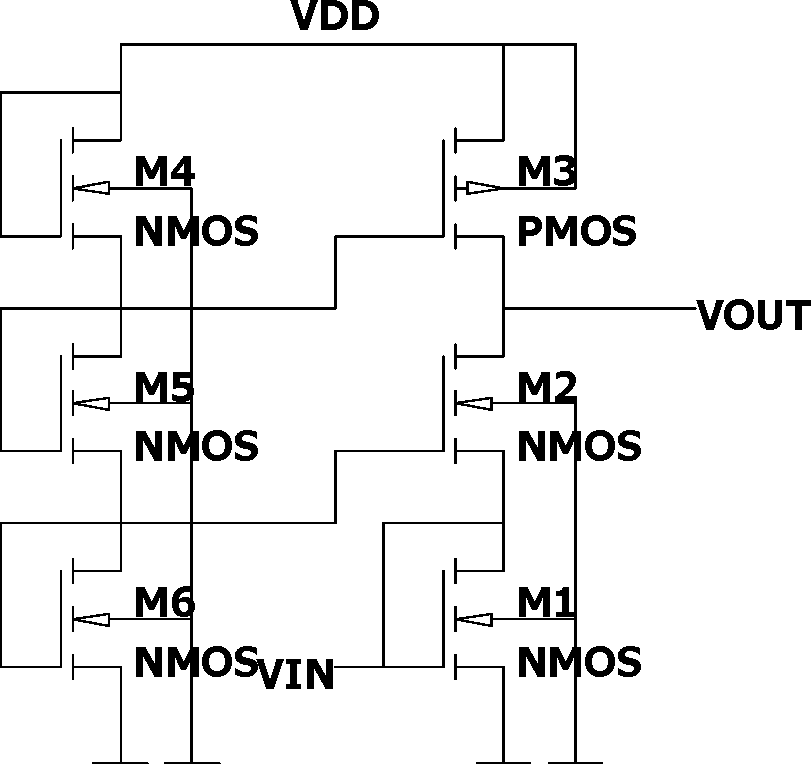
\includegraphics[height=6cm]{tarea_CS.pdf}
            \end{figure}            
        \end{column}
        \begin{column}{0.35\textwidth}
            Realice primero todos los cálculos teóricos que justifiquen su diseño.

            \vspace{3mm}
            Demuestre que el circuito funciona correctamente mediante dos simulaciones de SPICE: una del punto de operación y otra de la ganancia en CA.

            \vspace{3mm}
            Puede elegir la tensión de alimentación y configurar los modelos con $\lambda=0$ y $\gamma=0$.
        \end{column}
    \end{columns}

\end{frame}


\end{document}